\usepackage{booktabs}  % professionally typeset tables
\usepackage{amsmath}
\usepackage{amssymb}
\usepackage{textcomp}  % better copyright sign, among other things
\usepackage{xcolor}
\usepackage{lipsum}    % filler text
\usepackage{subfig}    % composite figures
\usepackage{url}
\usepackage{placeins}

\subsection{Surface reconstruction in the general case}
For some meshes, the requirement of global $C^2$ continuity is too restrictive. Also, a procedure similar to that described in the previous section would be quite expensive for surfaces in $\mathbb{R}^3$. We therefore consider local fittings of 2D Taylor polynomials at every boundary vertex, as described in \cite{sr:jiaowang} as ``Weighted Averaging of Local Fittings" (WALF). In their paper, Jiao and Wang fit local 2D Taylor polynomials to each vertex of the surface mesh. The coefficients, that is, the derivatives of a local height function in a local coordinate system centered at the vertex, are solved for using vertex position data from a neighborhood of that vertex. It is ensured that there are more neighboring points being considered for data than the number of unknowns to solve for, thereby obtaining an over-determined system of equations. This is solved by a weighted least-squares approach. We first describe the original method in \cite{sr:jiaowang}.

In Jiao and Wang's method, a local $uvw$ coordinate system is determined at each vertex of the surface mesh. How this is done is suggested in \cite{sr:diffquant} by Jiao and Zha. An estimate of the outward normal to the surface at the vertex serves as the $w$-axis of the local coordinate frame. Once the normal direction $\hat{\bld{n}}$ is decided, the $u$ direction is taken as any direction normal to the $w$-axis. Let the $u$ direction be along $\bld{t}_1$ in global coordinates. Finally, $\hat{\bld{t}_2} = \hat{\bld{n}} \times \hat{\bld{t}_1}$ forms the $v$ direction. Thus we obtain a right-handed $uvw$ coordinate system. We can transform any point with global coordinates $\bld{x}$ can be transformed to $\bld{u}$ in the local frame of the point at $\bld{x}_0$ as
\begin{equation}
\bld{u} = \bld{Q} (\bld{x} - \bld{x}_0)
\end{equation}
where
\begin{equation}
\bld{Q} =
\begin{bmatrix}
\hat{\bld{t}_1} & \vert & \hat{\bld{t}_2} & \vert & \hat{\bld{n}}
\end{bmatrix}
\end{equation}
is an orthogonal rotation matrix.

Next, a locally high-order surface is reconstructed by expanding a local height function in a Taylor polynomial around that vertex. For reconsucting a $d$-degree surface, the local height function $h$ is expressed as
\begin{equation}
h(u,v) \approx \sum_{i=0}^d \sum_{j\geq 0,k\geq 0}^{j+k \leq d} \frac{u^j v^k}{j!k!} D_{jk}
\end{equation}
where $D_{jk} := \frac{\partial^{j+k} h}{\partial^j u \, \partial^k v}$,
Suppose we consider $m$ linear mesh vertices around a vertex for the reconstruction at the latter vertex, we obtain a system of equations to solve for the derivatives $D_{jk}$. Thus we have an $m \times n$ system with $n:= \frac12 (d+1)(d+2)$, i.e.,
\begin{equation}
\sum_{i=0}^d \sum_{j\geq 0,k\geq 0}^{j+k \leq d} \frac{u_p^j v_p^k}{j!k!} D_{jk} \approx h_p
\label{eq:sr_taylorequation}
\end{equation}
for $p \in \{1,2,...,m \}$. If $m \ge n$, this system can be solved in a least-squares sense. We can write the system of equations as
\begin{equation}
\bld{V} \bld{D} = \bld{f}
\end{equation}
where $\bld{V} (m\times n)$ is the generalized Vandermonde matrix for 2D Taylor polynomials, $\bld{D}$ is the $n$-vector of derivatives of the height function at the local origin, and $\bld{f}$ is the $m$-vector of heights of points in the reconstruction stencil. The system is solved by a weighted least-squares method. This is done for each vertex on the boundary.

For each vertex, the reconstruction stencil is selected according to the degree of polynomial surface required. It is claimed \cite{sr:diffquant} that $m$ should be from 1.5 to 2 times $n$. A general method for selecting reconstruction stencils for triangular and rectangular surface meshes is given by Jiao and Wang \cite{sr:jiaowang}. Here, we are mainly concerned with obtaining good P2 discretizations, for which the stencil is shown in figure \ref{f:stencil}. All vertices shown are used in reconstructing the surface at the center vertex.

\begin{figure}
	\centering
	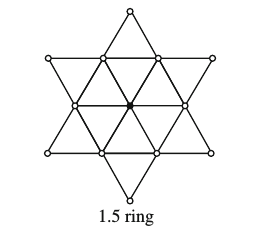
\includegraphics[scale=1.0]{stencil}
	\caption{Stencil for reconstruction of P2 surface; from \cite{sr:jiaowang}}
	\label{f:stencil}
\end{figure}

The weighted least-squares problem is expressed as
\begin{equation}
\min_{\bld{D}} \lVert \bld{W}(\bld{V}\bld{D}-\bld{f})\rVert_2
\label{eq:sr_wls}
\end{equation}
where $\bld{W}$ is an $m \times m$ diagonal weighting matrix. The weight for the $i$th point in the stencil is taken as (see \cite{sr:diffquant})
\begin{eqnarray}
w_i &=& \frac{\gamma_i^+}{(\sqrt{\lVert\bld{u}_i\rVert^2 + \epsilon})^{d/2}} \, , \text{where} \\
\gamma_i^+ &=& \max\{0,\hat{\bld{n}_i}^ T\hat{\bld{n}_0}\}, \\
\epsilon &=& \frac{1}{100m} \sum_{i=1}^m \lVert\bld{u}_i \rVert^2.
\label{eq:sr_weight}
\end{eqnarray}
In the above equations, $\bld{u}_i$ and $\hat{\bld{n}_i}$ denote the position of and normal at the $i$ vertex in the reconstruction stencil, respectively, while $\hat{\bld{n}_0}$ denotes the normal at the vertex for which the local reconstruction is being computed.

The least-squares problem is solved by a QR factorization method using Householder transformations. Once the coefficients $\bld{D}$ are found for each point, we can move the high-order nodes accordingly.

For the case of surface reconstruction of the unstructured mesh of a sphere, we observe that the method described above does not work very well. Since vertex normals are required for determining the local coordinate frames and for the weights of the least-squares formulation, we need to estimate them. It turns out that the quality of the reconstruction is \emph{very} sensitive to the accuracy of the point normal. If the vertex normal is chosen as a simple average of face normals, there are large errors in some places on the reconstructed surface. The normal can also be estimated as a weighted average of the face-normals of the faces surrounding the vertex. We use either an inverse-distance weighted average or an area-weighted average. In this case, the results are better, but mostly still unusable. 
